\section{Angular basis}
\label{sec:kstmm:basis}

The differential angular distribution for \BdToKstll is expressed as a
function of  five kinematic variables: three angles (\ctl, \ctk, $\phi$) 
and two invariant masses;
the mass squared of the \kpi system is denoted \psq and the 
mass squared of the dilepton pair (\qsq),  
the angle $\theta_K$ is defined as the angle between the \Kp and the \B momentum
vector in the rest frame of the \Bd.  The angle $\theta_\ell$ is
 defined as the one between the \ellp in the rest frame of the dilepton
pair and the momentum vector of the \Bd.  The angle $\phi$ is defined
as the signed angle between the planes formed by the dilepton pair and the \kpi pair respectively, 
in the rest frame of the \Bd.\footnote{This is the same sign convention for \ctl as used in all 
previous experiments and the same $\phi$ convention as used in 
\lhcb~\cite{Aaij:2013iag}.}

For the \CP-conjugate decay \BdbToKstbll, $\theta_\ell$ is defined with respect to the \ellm instead of the \ellp
and $\theta_K$ is defined with respect to the \Km instead of the \Kp.
There are two possible definitions of $\phi$, a \CP symmetric definition which 
changes through a minus sign and a \CP anti-symmetric definition, \phiacp, 
which is unchanged between the \Bd and \Bdb decay. 
An illustration of the angles for \BdbToKstbll is shown in Fig~\ref{fig:kstmm:angles}.
\begin{figure}[tbp]
\centering
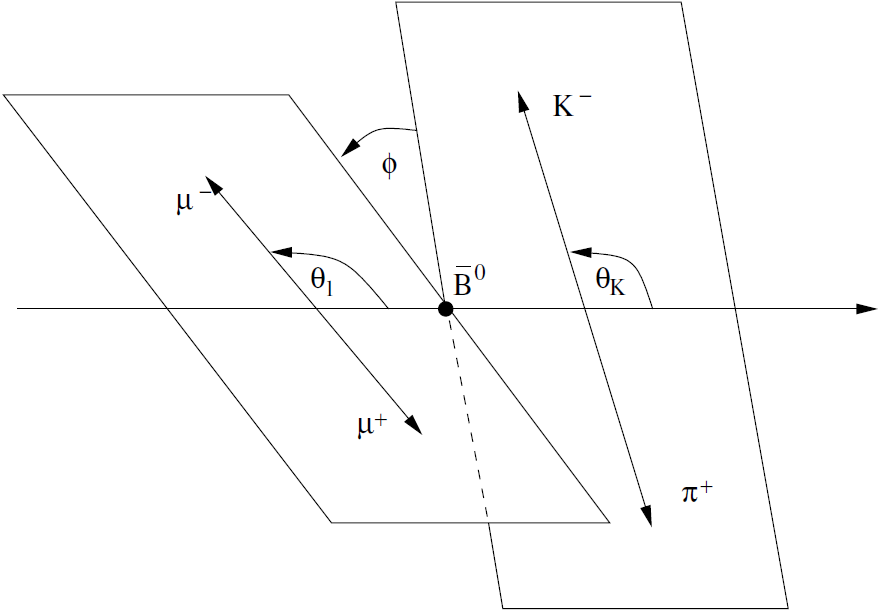
\includegraphics[width=0.48\columnwidth]{chapter4/figs/restMassAngles.png}
\caption[An illustration of the angles used to describe the \BdbToKstbll decay.]
{An illustration of the angles used to describe the \BdbToKstbll decay.
 The angle $\theta_l$ is defined between the \ellm and the \Bdb in the dilepton rest frame.
 The angle $\theta_K$ is defined between the \Km and the \Bdb in the \kpi rest frame.
 The angle $\phi$ is the signed angle between $\ellm$ and $\Km$ in the rest frame of the \Bdb. 
~\label{fig:kstmm:angles} }
\end{figure}

The angles \ctl and \ctk are given explicitly as 
\begin{align}
\ctl = \left( \frac{ \vec{p}_{\ellp} \cdot \vec{p}_{\ellell}  }{|\vec{p}_{\ellp}||\vec{p}_{\ellell}|} \right), \quad 
\ctk = \left( \frac{ \vec{p}_{\Kp} \cdot \vec{p}_{\kpi}  }{|\vec{p}_{\Kp}||\vec{p}_{\kpi}|}  \right) \, ,
\end{align}
where each momentum vector $\vec{p}$ is defined in the rest frame of the parent particle, i.e. 
the lepton momentum, $\vec{p}_{\ellp}$, is in the dilepton rest frame and dilepton momentum, $\vec{p}_{\ellell}$, is in \Bd rest frame.
The angle $\phi$ is calculated as %the difference between the angles $\theta_\ell$ and $\theta_K$ and
\begin{align}
\cos\phi &=    \left( \frac{\vec{p}_{\ellp} \times \vec{p}_{\ellm} }{|\vec{p}_{\ellp} \times \vec{p}_{\ellm}|} \right) \cdot 
   \left( \frac{\vec{p}_{\Kp} \times \vec{p}_{\pim} }{|\vec{p}_{\Kp} \times \vec{p}_{\pim}|} \right)  \, .
\end{align}
%and
%\begin{align}
%\sin\phi =    \left(\frac{ \vec{p}_{\ellp} \times \vec{p}_{\ellm} }{|\vec{p}_{\ellp} \times \vec{p}_{\ellm}|} \right) \times 
%   \left(\frac{ \vec{p}_{\Kp} \times \vec{p}_{\pim} }{|\vec{p}_{\Kp} \times \vec{p}_{\pim}|} \right) 
%   \cdot \frac{\vec{p}_{\kpi}}{|\vec{p}_{\kpi}|}  \, .
%\end{align}
For the CP-conjugate \BdbToKstbll decay, the angles \ctl and \ctk are given explicitly as 
\begin{align}
\cos\theta_{\bar{\ell}} &= \left( \frac{ \vec{p}_{\ellm} \cdot \vec{p}_{\ellell}  }{|\vec{p}_{\ellm}||\vec{p}_{\ellell}|} \right), \quad 
\cos\theta_{\bar{K}} = \left( \frac{ \vec{p}_{\Km} \cdot \vec{p}_{\kpi}  }{|\vec{p}_{\Km}||\vec{p}_{\kpi}|}  \right) \, ,
\end{align}
and applying the \CP operator to the definition of $\phi$ gives the relation,
\begin{align}
\cos\phi &= \left( \frac{\vec{p}_{\ellm} \times \vec{p}_{\ellp} }{|\vec{p}_{\ellm} \times \vec{p}_{\ellp}|} \right) \cdot 
   \left( \frac{\vec{p}_{\Km} \times \vec{p}_{\pip} }{|\vec{p}_{\Km} \times \vec{p}_{\pip}|} \right)  \, . 
\end{align}
The \CP anti-symmetric definition of $\phi$ is given by only applying the \CP operator to the \kpi state, 
\begin{align}
\cos\phiacp &= \left( \frac{\vec{p}_{\ellp} \times \vec{p}_{\ellm} }{|\vec{p}_{\ellp} \times \vec{p}_{\ellm}|} \right) \cdot 
   \left( \frac{\vec{p}_{\Km} \times \vec{p}_{\pip} }{|\vec{p}_{\Km} \times \vec{p}_{\pip}|} \right)  \, .
\end{align}

Each of the angles are defined over the intervals
\begin{align}
0 \leq \theta_{\textit{l}} < \pi, \quad 0 \leq \theta_{\textit{K}} < \pi, \quad -\pi \leq \phi < \pi,
\end{align}
such that the angular distribution is defined over the range
\begin{align}
-1 \leq \ctl < 1, \quad -1 \leq \ctk < 1, \quad -\pi < \phi < \pi \, .
\end{align}
